\section{Finite State Machines}

FSM consists of states and transitions.
State machiens are used for modeling systems that have a finite number
of states and whose behavior is determined by the current state and
the input. The states are drawn as circles and the transitions are
drawn as arrows between the states. The transitions are labeled with
the input that causes the transition.
State machines can be made using two models: Mealy and Moore. In
Mealy state machines, the output
is a function of the current state and the input.
When the input change, the outputs are updated without waiting for a clock
edge. The mealy state machine is represented in the following figure:

\begin{center}
	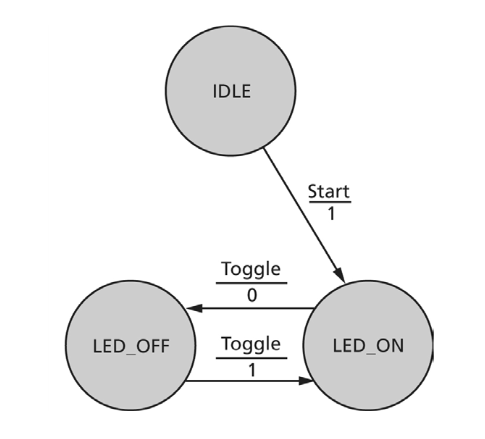
\includegraphics[width=0.3\textwidth]{images/mealy.png}
\end{center}

In Moore state the output is a function of the current state only.
The outputs are only written when the state changes (on clock edge).
The moore state machine is shown on the following figure:

\begin{center}
	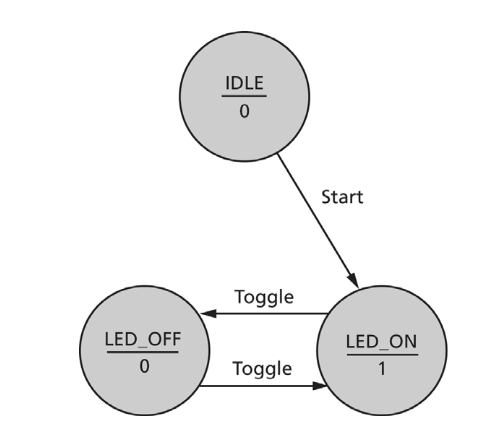
\includegraphics[width=0.3\textwidth]{images/moore.png}
\end{center}


The hardware representation of a state machine can be visualized as:

\begin{center}
	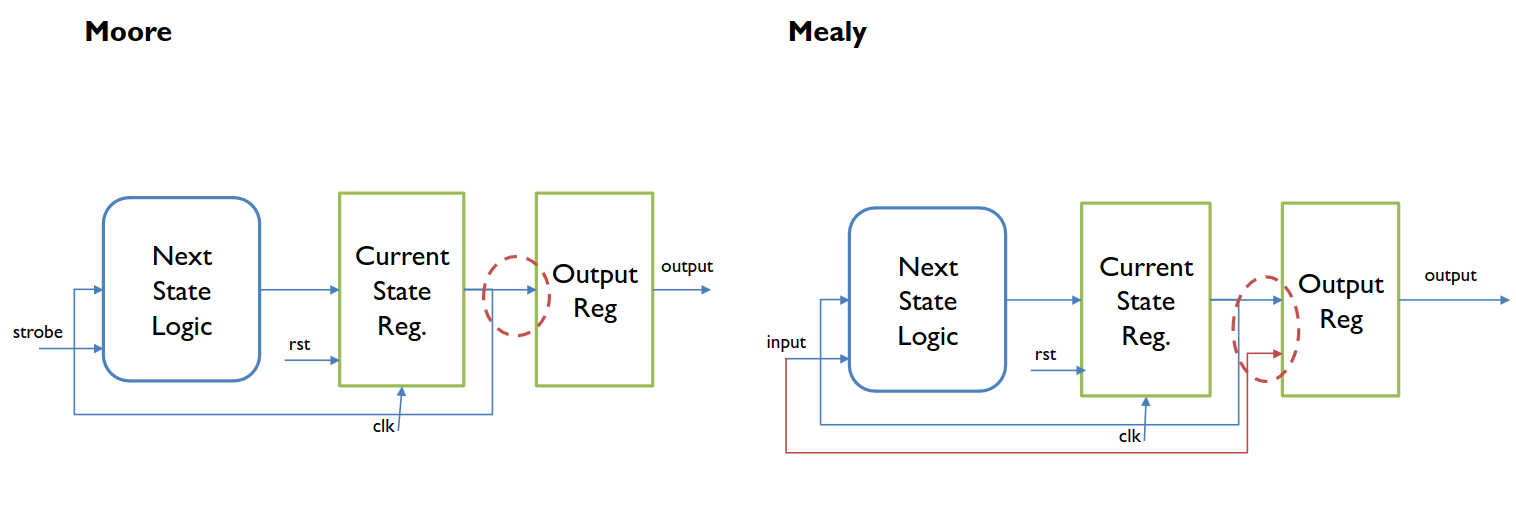
\includegraphics[width=0.9\textwidth]{images/fsm_hardware.png}
\end{center}

